\appendix 

\section{付録}
\label{appendix}
\subsection{使用した部屋の外見、見取り図}

\newpage

\subsection{実験で使用した機器の仕様表}

\begin{table}[ht]
\caption{Specifications of the dual-arms robots}    
\centering
  \begin{tabular}{ll} \hline
    Specification & Value / Type \\ \hline 
    Model & HIRO-NX  \\ 
    Number of controlled axes & 15 (Neck:2, Arm:6($\times$2), Waist:1)  \\
    Pose repeatability & $\pm$0.01 mm \\
    Related payload & 1.5 kg (both hand 3 kg) \\ 
    Weight & 28 kg   \\ \hline 
  \end{tabular}
  \label{tab:deformasion_1}
\end{table}

\begin{table}[ht]
\caption{Specifications of the robotic hand}    
\centering
  \begin{tabular}{ll} \hline
    Specification & Value / Type \\ \hline 
    Model & TRX-S  \\ 
    Fingertip force & 10 N  \\
    Grasping force & 30 N  \\  
    Load capacity & 3 kg \\ 
    Weight & 320 g   \\ 
    Grasping diameter & 10 - 100 mm  \\ 
    Actuator & Stepping motor with ball screw   \\ \hline 
  \end{tabular}
  \label{tab:deformasion_2}
\end{table}


\begin{table}[ht]
\caption{Specifications of the force (tactile) sensor}    
\centering
  \begin{tabular}{ll} \hline
    Specification & Value / Type \\ \hline 
    Model & OMD-20-SE-40N  \\ 
    Nominal capacity & ($f_z$): 40 N  \\
      & ($f_x,f_y$): $\pm$20 N  \\
    Typical deformation & ($f_z$): 2 mm  \\
      & ($f_x,f_y$): 1.5 mm  \\
    Grasping force & $17\times25\times25$ mm$^3$  \\  
    Weight (with 1 m cable) & 23 g   \\ 
    Maximum sampling freqency & 100 Hz   \\ \hline 
  \end{tabular}
  \label{tab:deformasion_3}
\end{table}

\clearpage

\subsection{使用した対象物体の外観}

\begin{figure}[ht]
\centering
\subfigure[Front view]{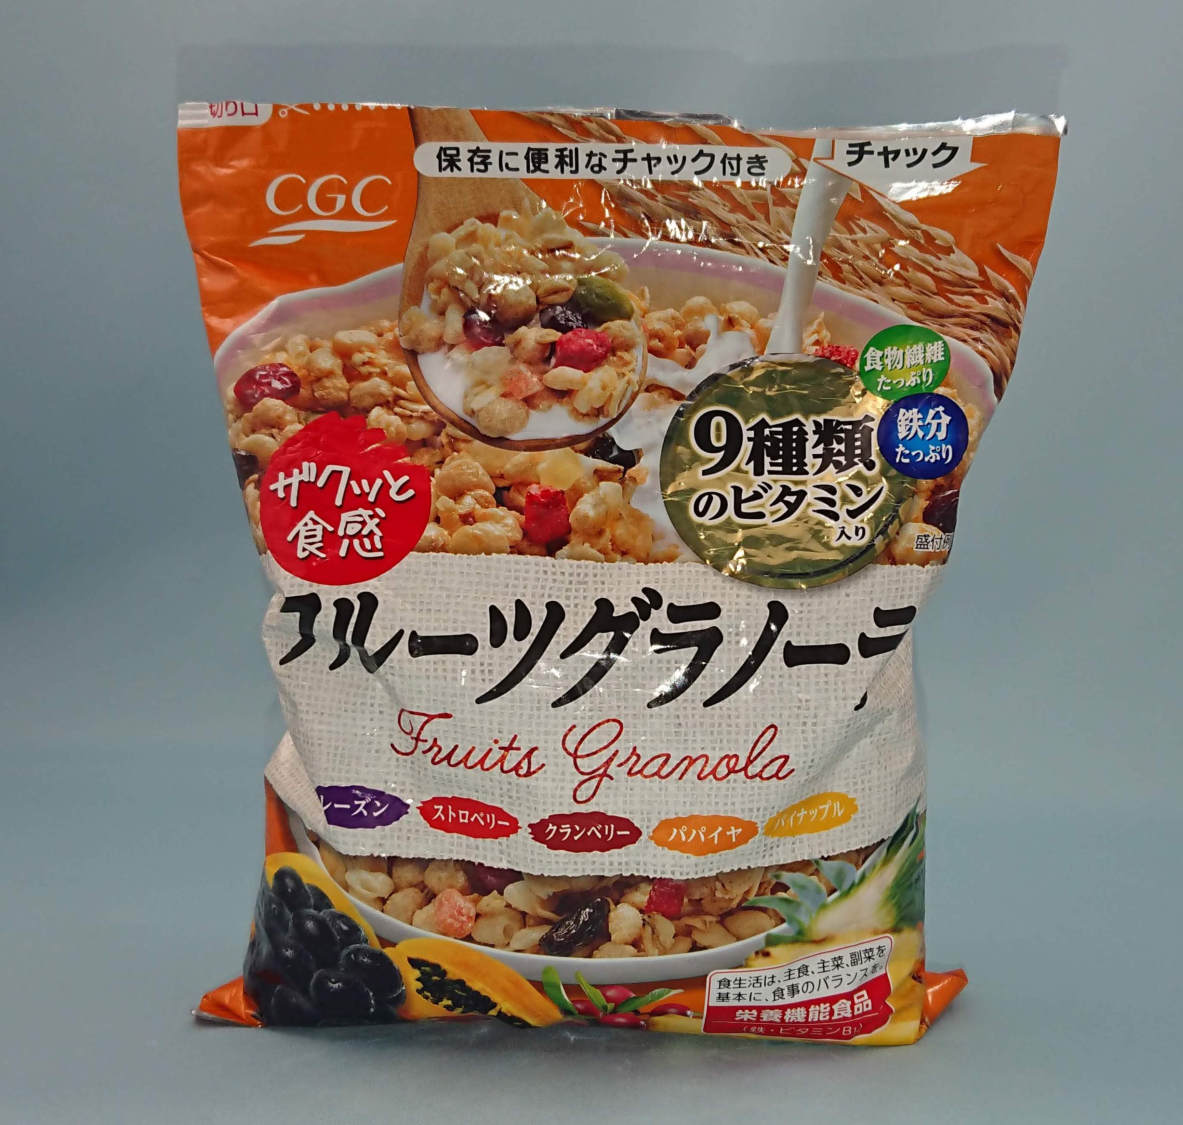
\includegraphics[width=0.40\linewidth]{images/cereal_front.pdf}
 \label{fig:cereal_front}} 
\subfigure[Left side view]{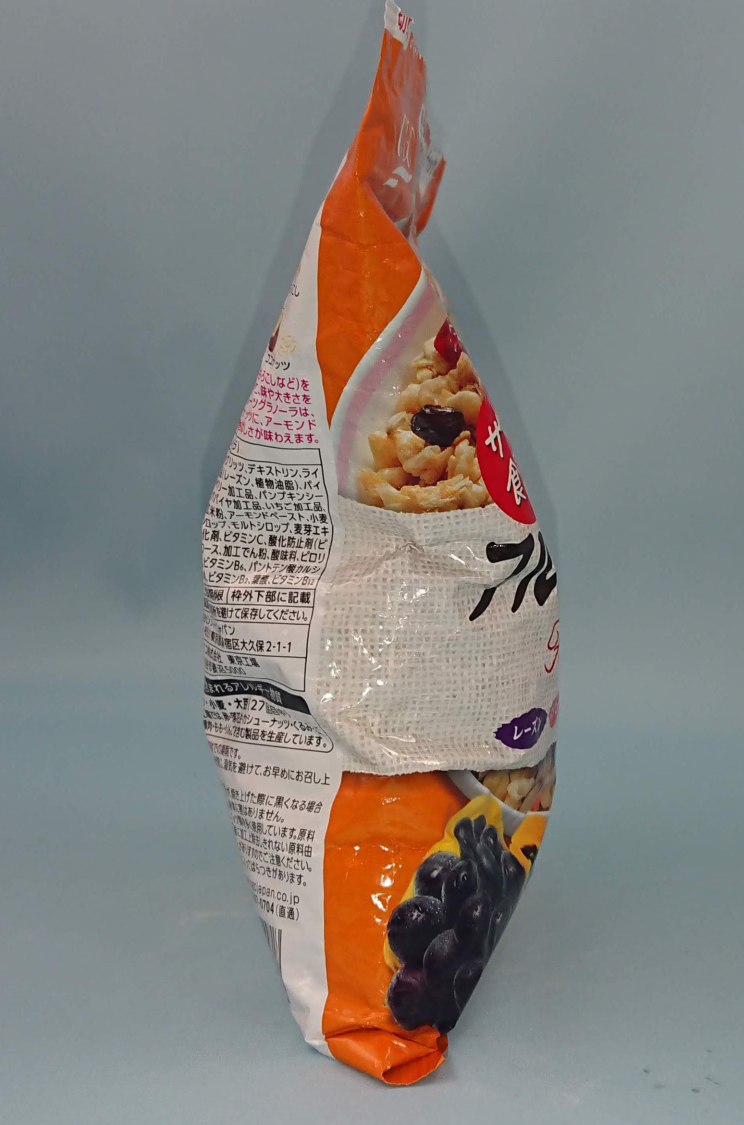
\includegraphics[width=0.25\linewidth]{images/cereal_leftside.pdf}
 \label{fig:cereal_leftside}} 
\subfigure[Right side view]{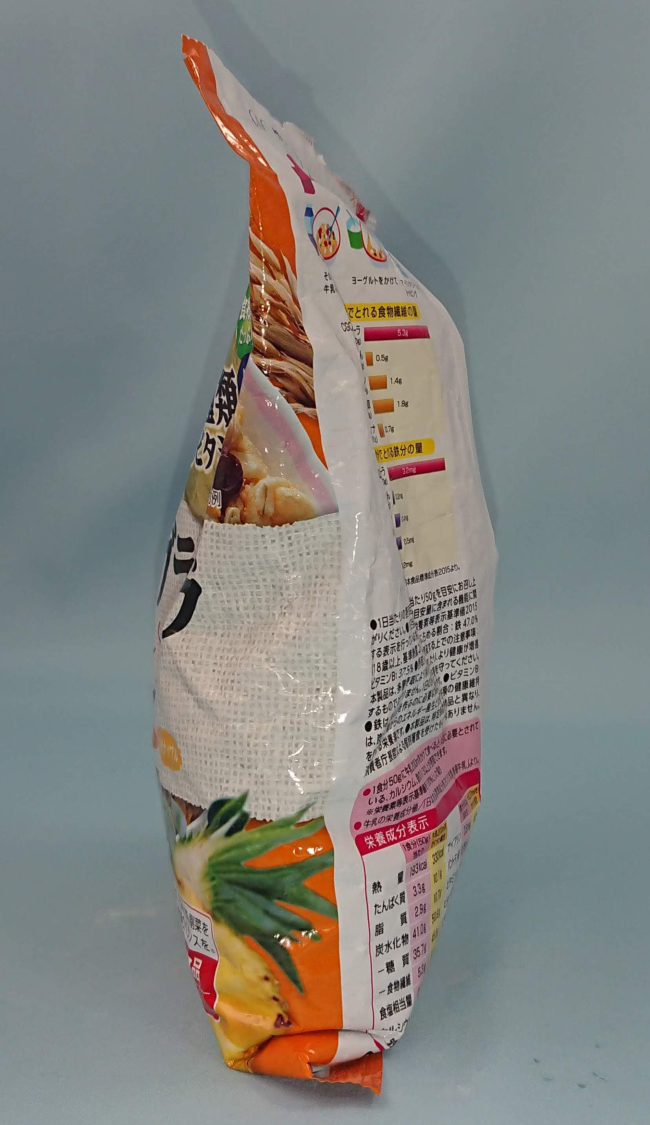
\includegraphics[width=0.22\linewidth]{images/cereal_rightside.pdf}
 \label{fig:cereal_rightside}} \\ 
\subfigure[Back view]{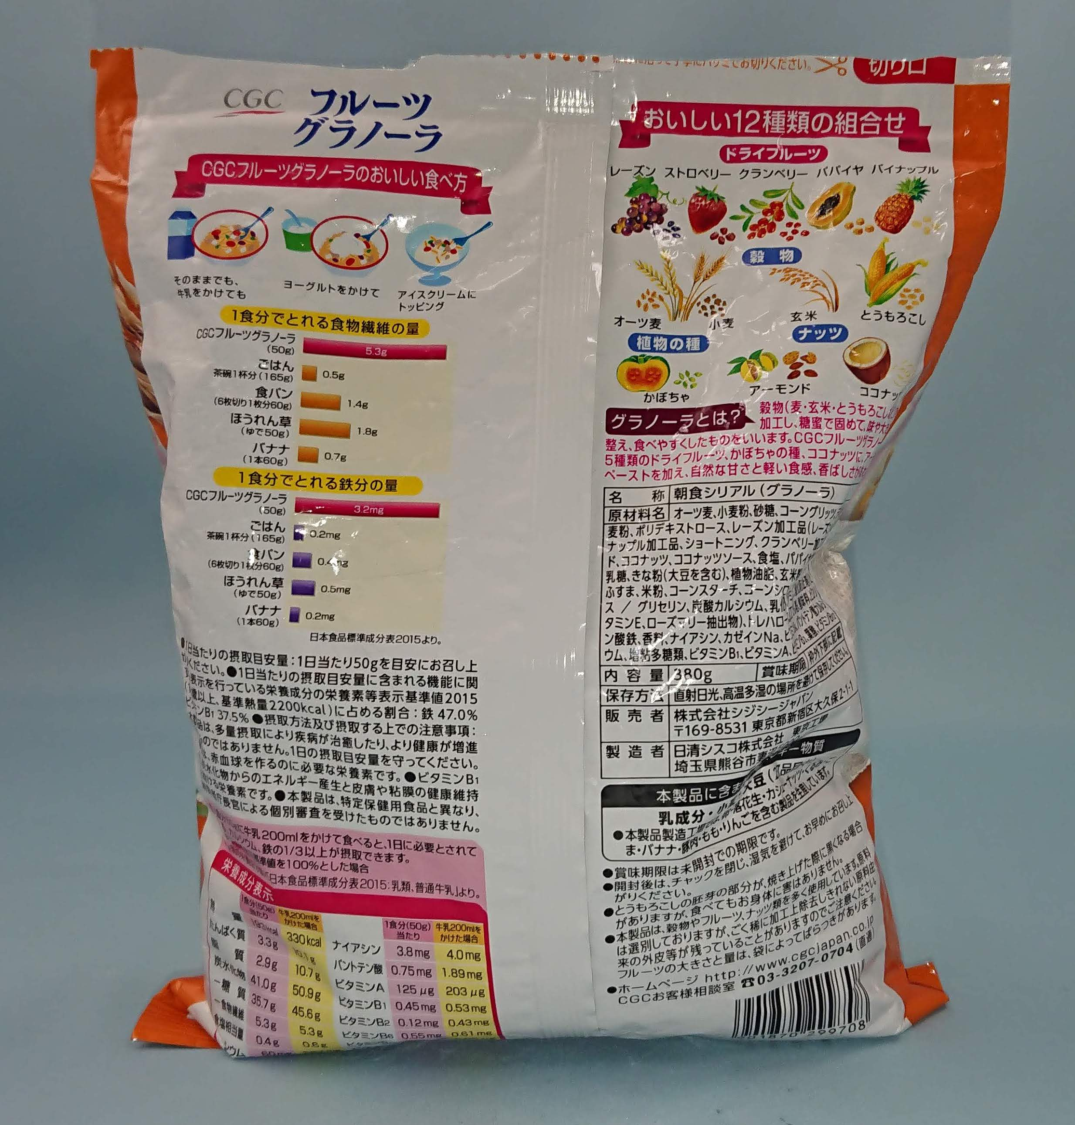
\includegraphics[width=0.46\linewidth]{images/cereal_back.pdf}
 \label{fig:cereal_back}}  
\subfigure[Top view]{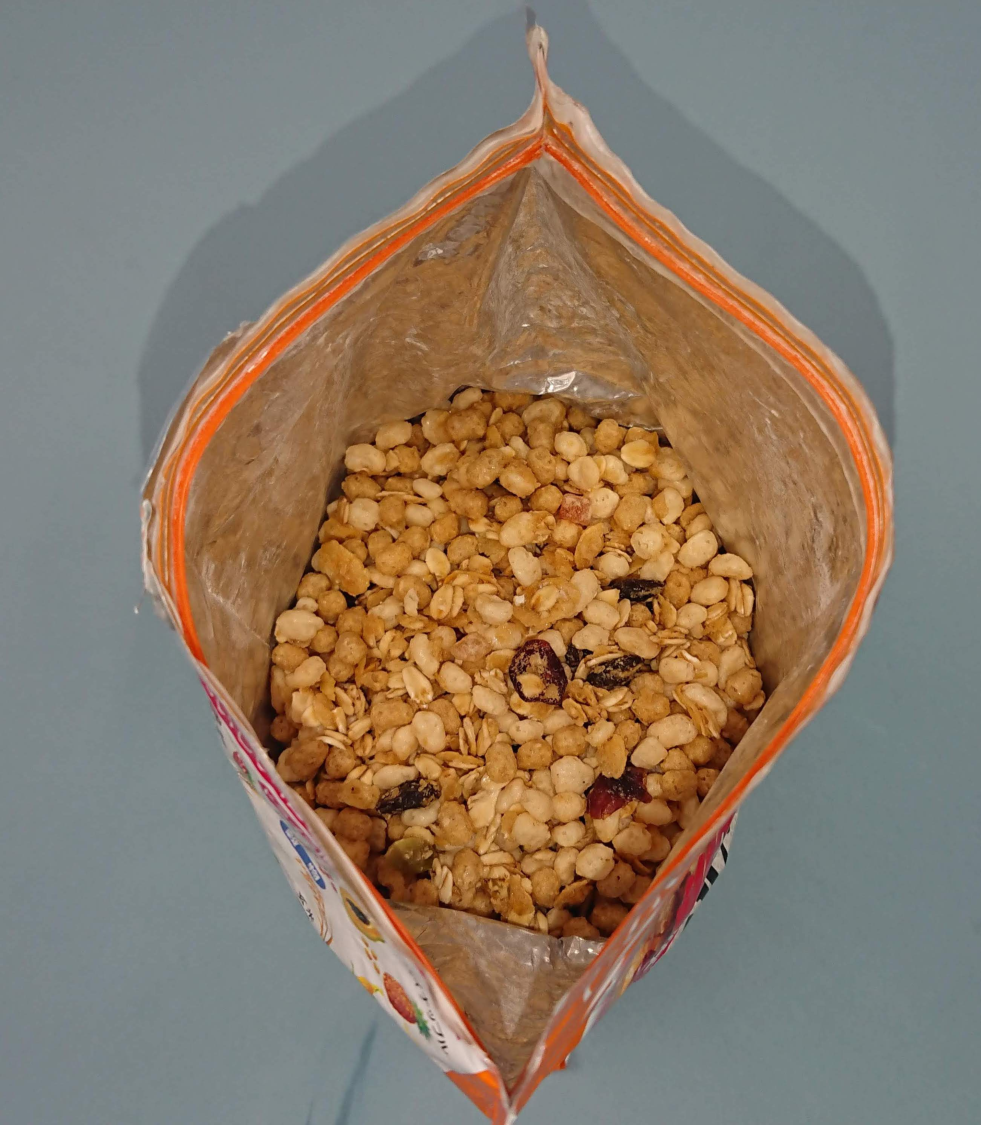
\includegraphics[width=0.42\linewidth]{images/cereal_top.pdf}
 \label{fig:cereal_top}}  
\caption{Appearance of breakfast cereal}
\label{fig:Breakfast_cereal}
\end{figure}

\begin{figure}[ht]
\centering
\subfigure[Front view]{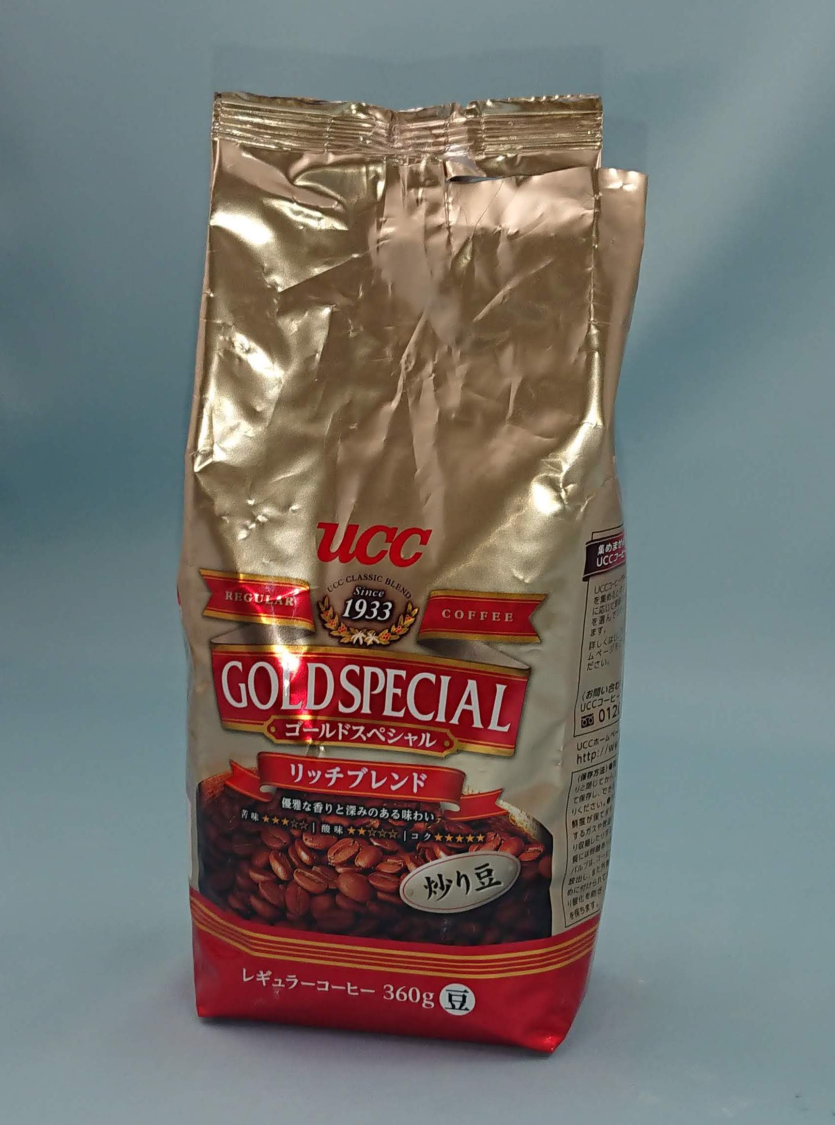
\includegraphics[width=0.36\linewidth]{images/coffee_front.pdf}
 \label{fig:coffee_front}} 
\subfigure[Left side view]{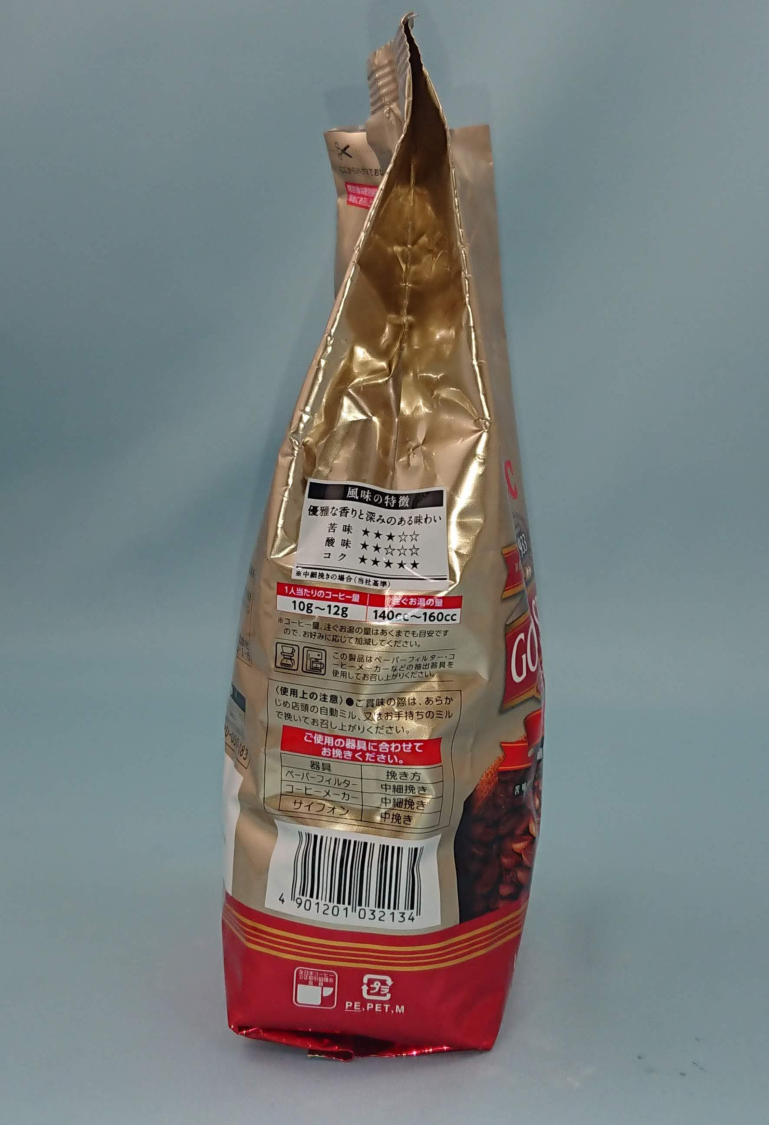
\includegraphics[width=0.32\linewidth]{images/coffee_leftside.pdf}
 \label{fig:coffee_leftside}} 
\subfigure[Right side view]{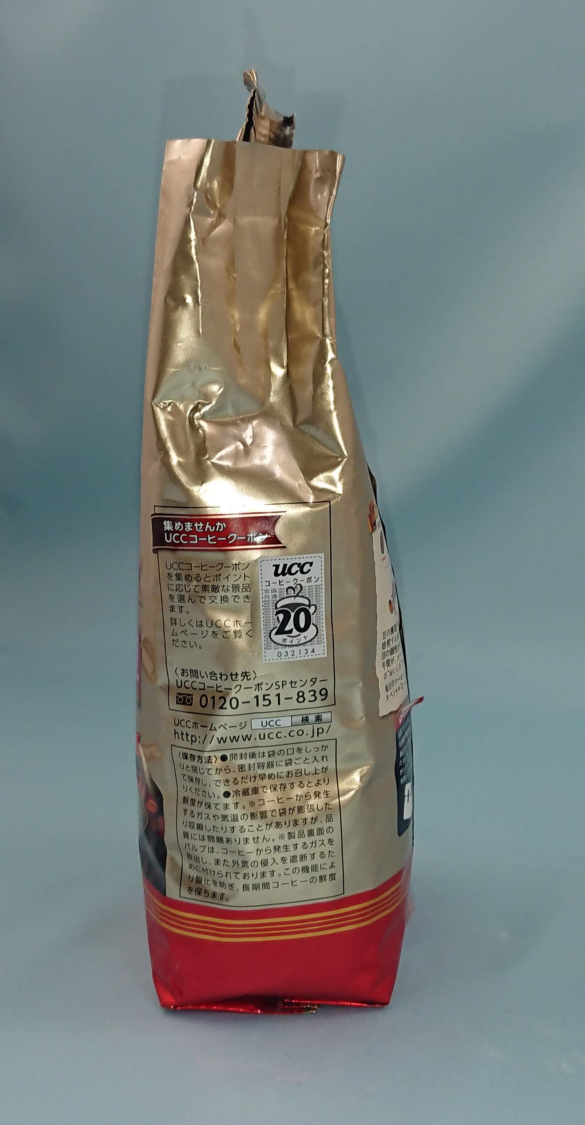
\includegraphics[width=0.24\linewidth]{images/coffee_rightside.pdf}
 \label{fig:coffee_rightside}} \\ 
\subfigure[Back view]{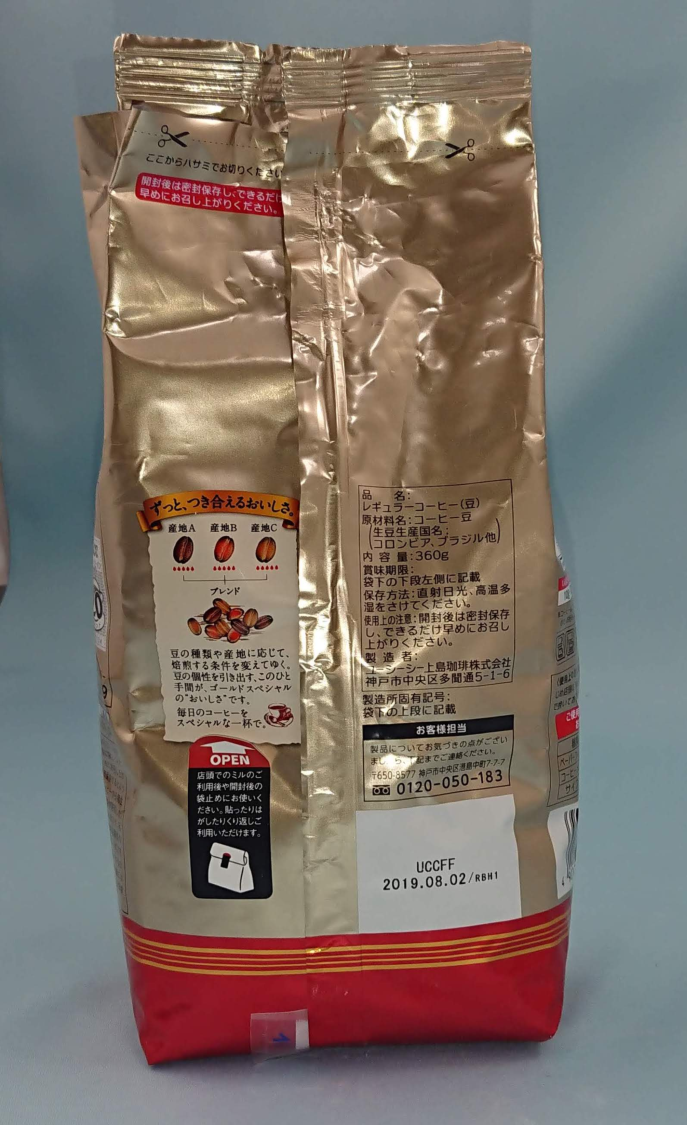
\includegraphics[width=0.34\linewidth]{images/coffee_back.pdf}
 \label{fig:coffee_back}}  
\subfigure[Top view]{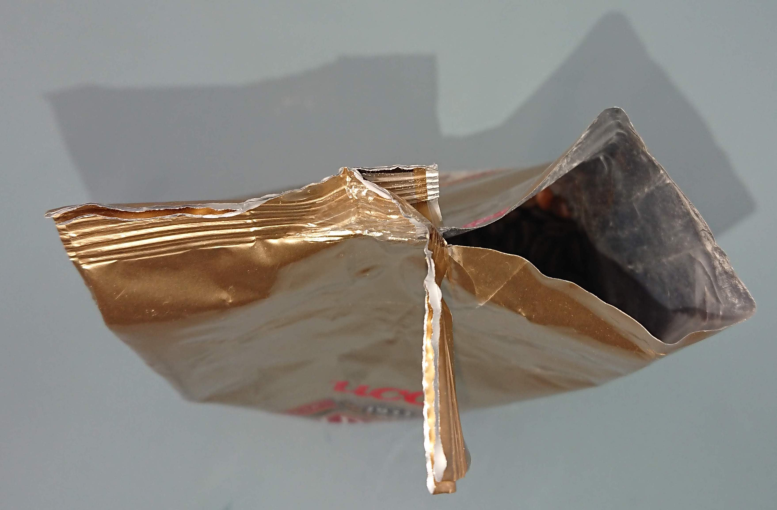
\includegraphics[width=0.52\linewidth]{images/coffee_top.pdf}
 \label{fig:coffee_top}}  
\caption{Appearance of coffee beans}
\label{fig:Coffee_beans}
\end{figure}


\begin{figure}[ht]
\centering
\subfigure[Front view]{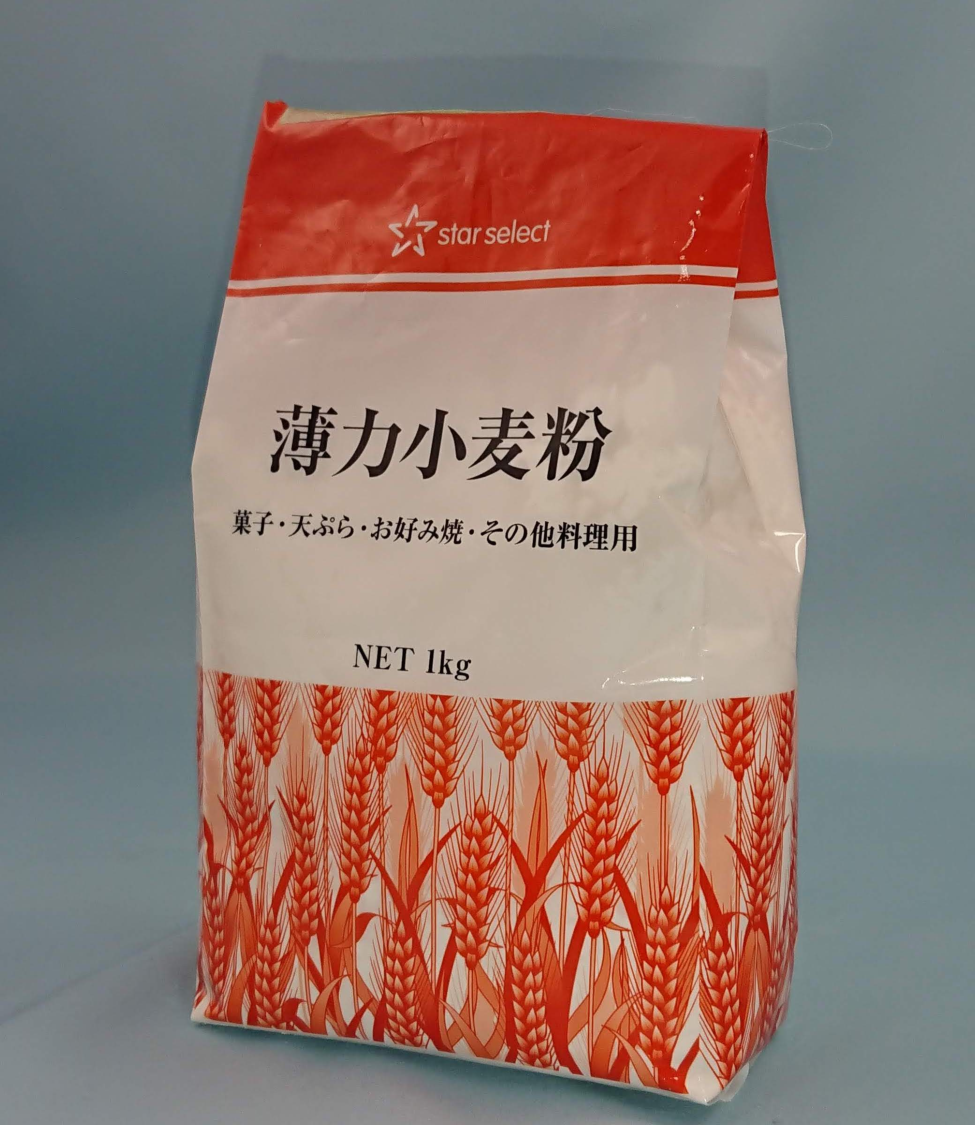
\includegraphics[width=0.42\linewidth]{images/flour_front.pdf}
 \label{fig:flour_front}} 
\subfigure[Left side view]{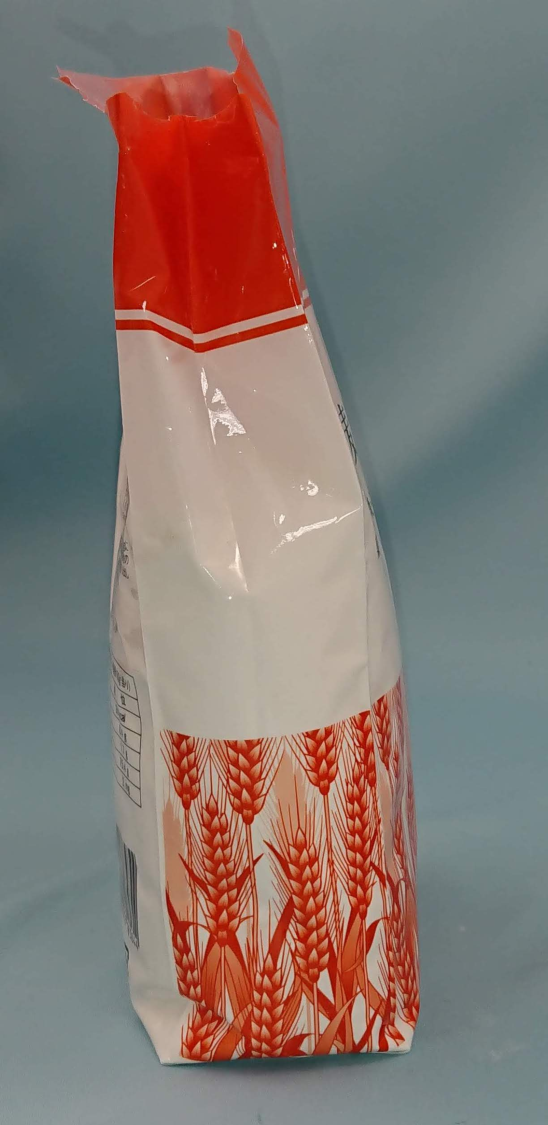
\includegraphics[width=0.23\linewidth]{images/flour_leftside.pdf}
 \label{fig:flour_leftside}} 
\subfigure[Right side view]{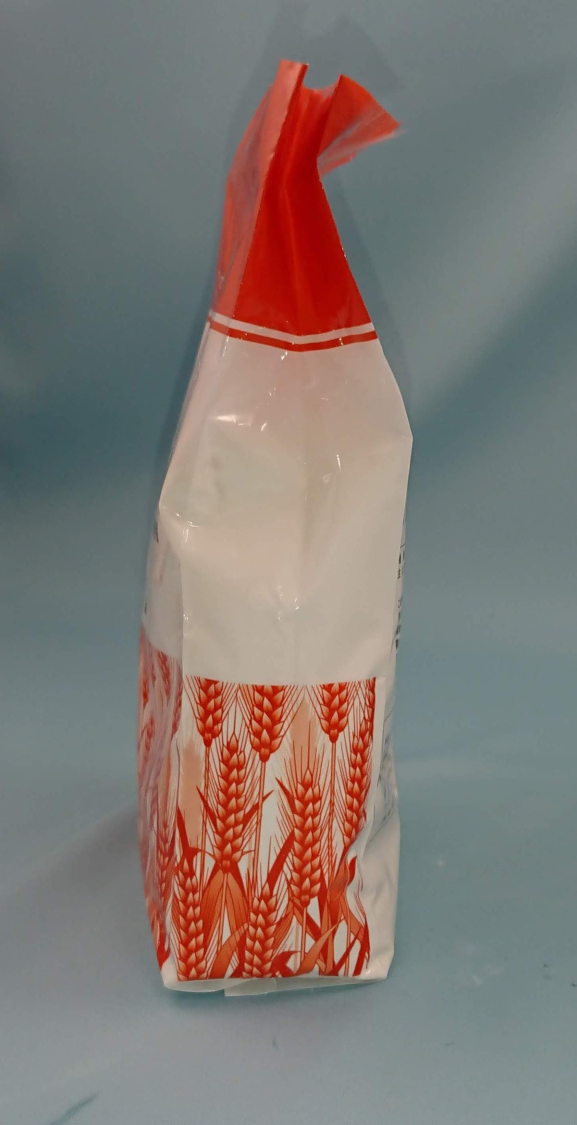
\includegraphics[width=0.24\linewidth]{images/flour_rightside.pdf}
 \label{fig:flour_rightside}} \\  
\subfigure[Back view]{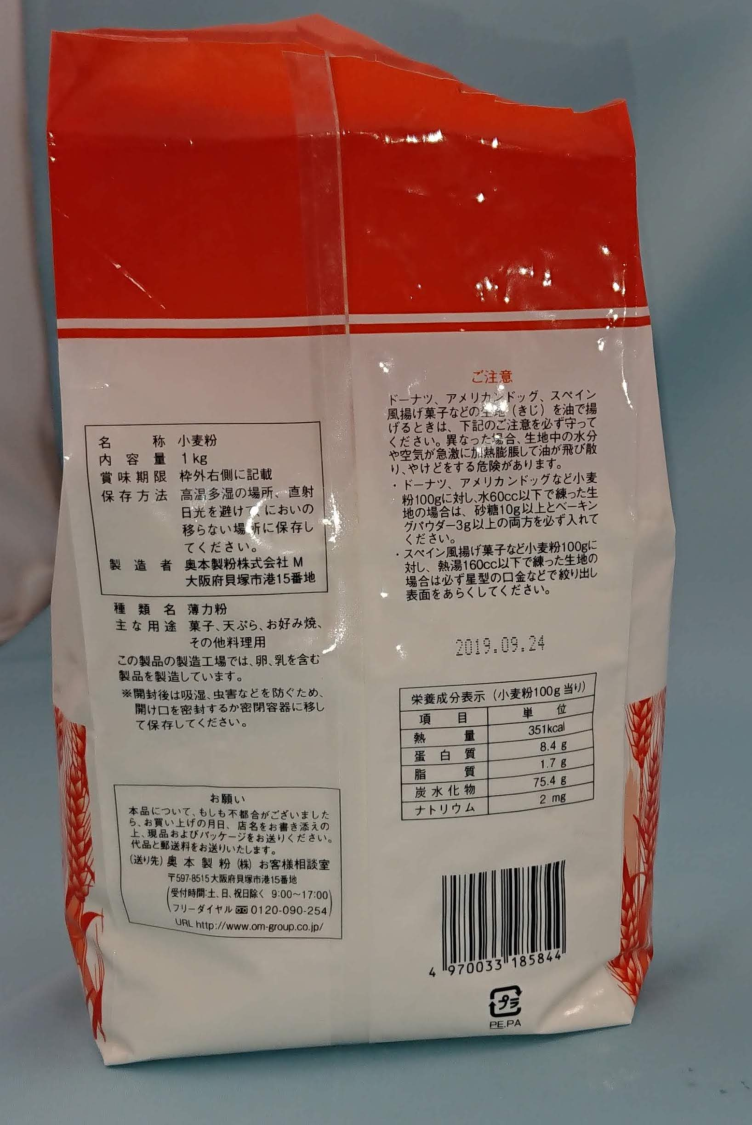
\includegraphics[width=0.34\linewidth]{images/flour_back.pdf}
 \label{fig:flour_back}}  
\subfigure[Top view]{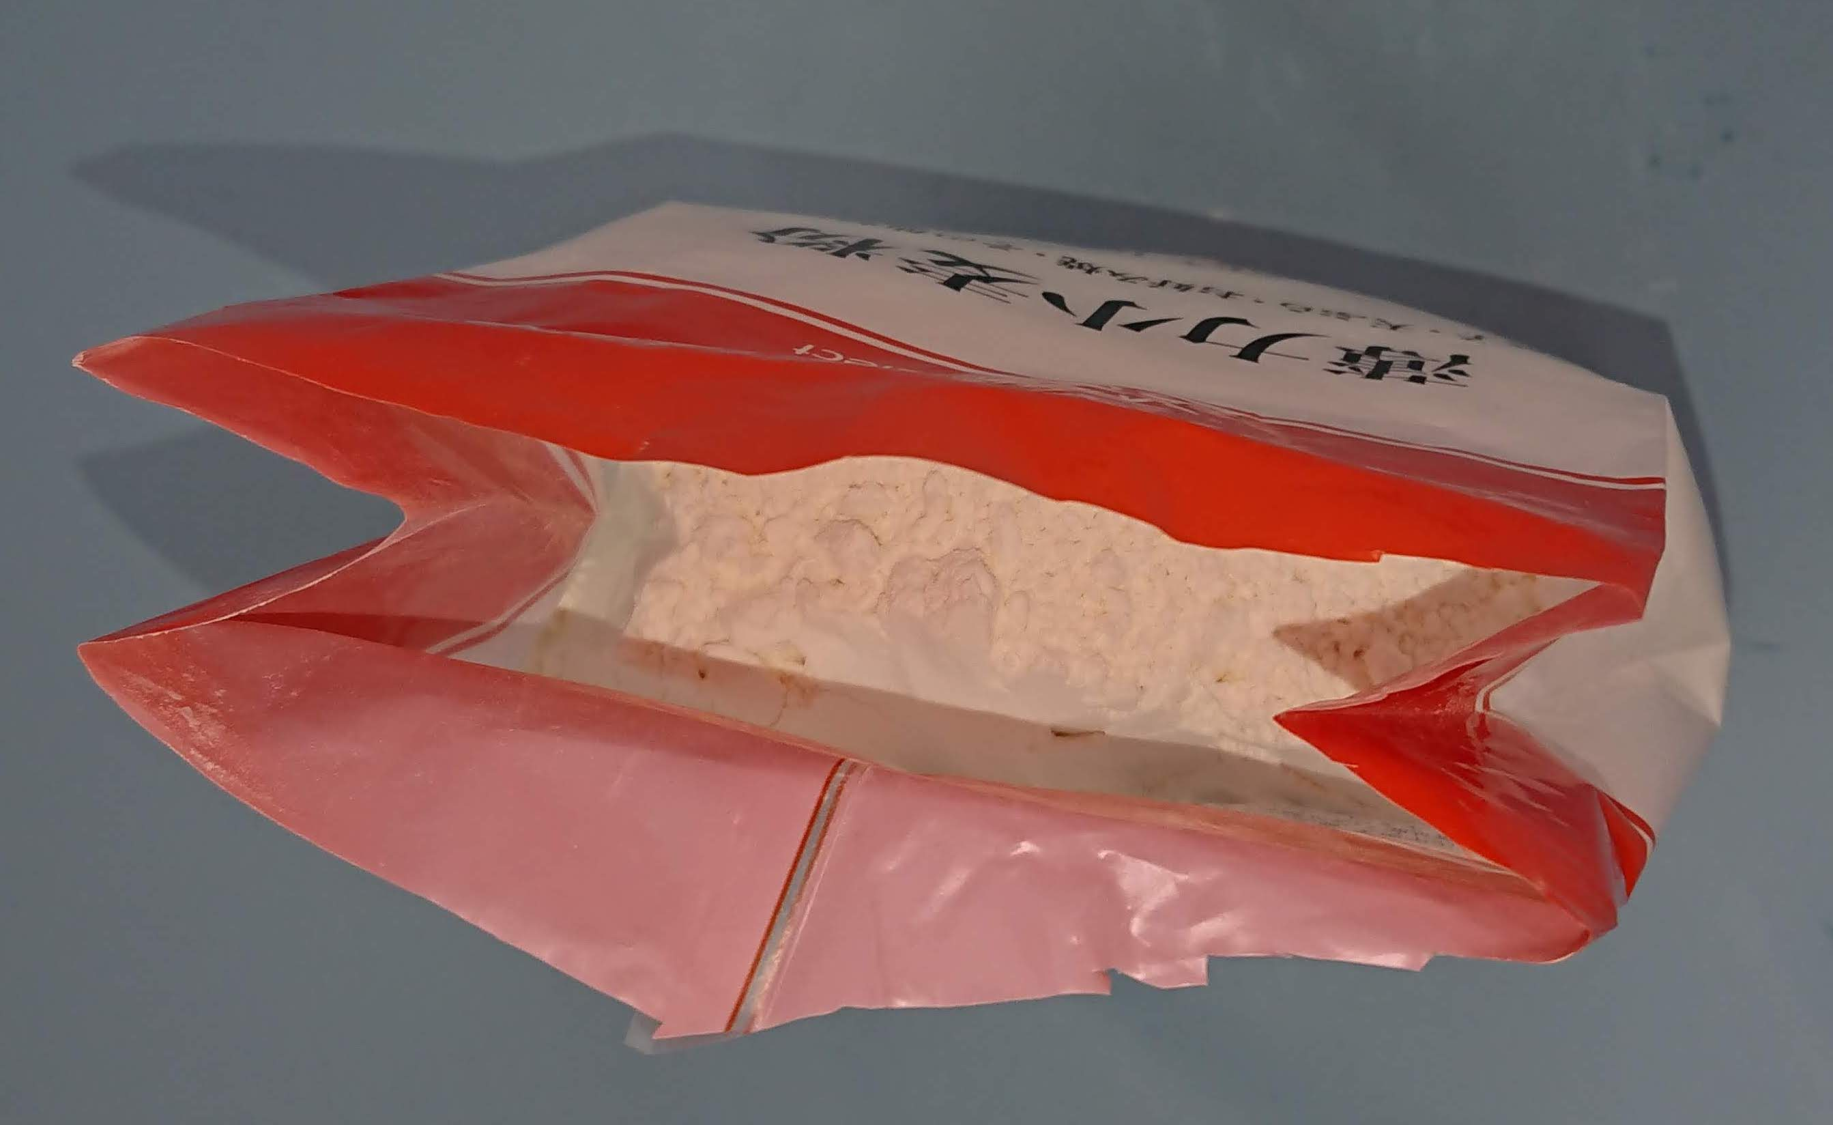
\includegraphics[width=0.50\linewidth]{images/flour_top.pdf}
 \label{fig:flour_top}}  
\caption{Appearance of flour}
\label{fig:flour}
\end{figure}

\begin{figure}[ht]
\centering
\subfigure[Front view]{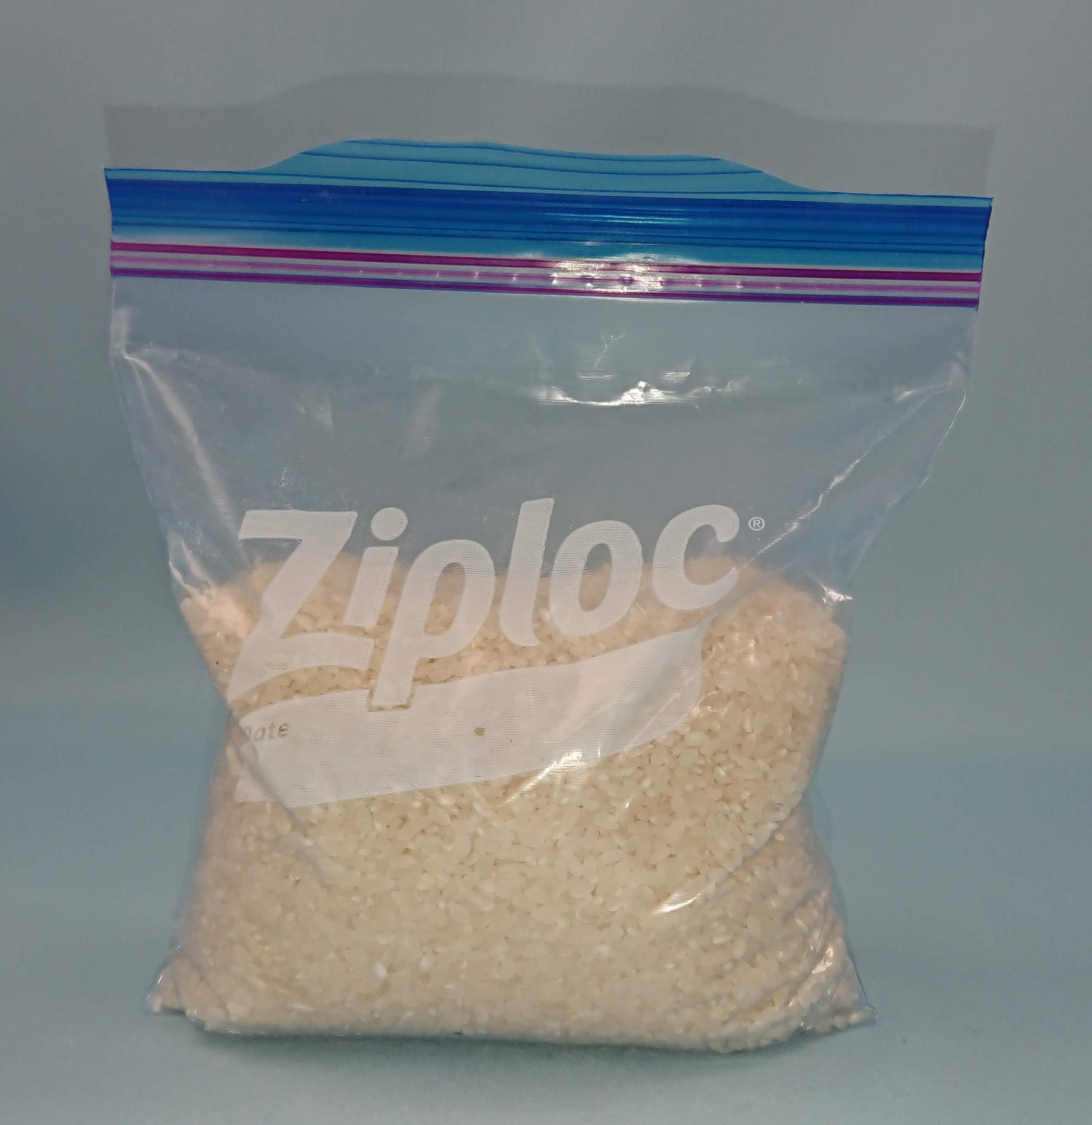
\includegraphics[width=0.40\linewidth]{images/rice_front.pdf}
 \label{fig:rice_front}} 
\subfigure[Left side view]{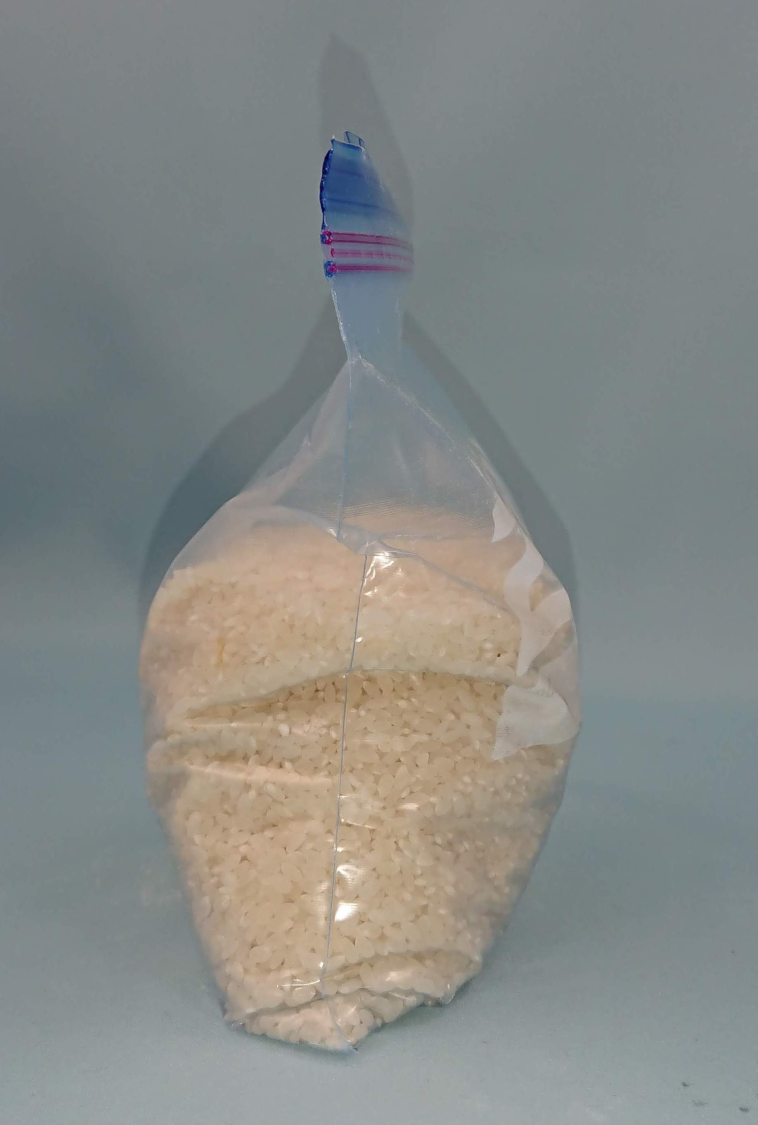
\includegraphics[width=0.27\linewidth]{images/rice_leftside.pdf}
 \label{fig:rice_leftside}} 
\subfigure[Right side view]{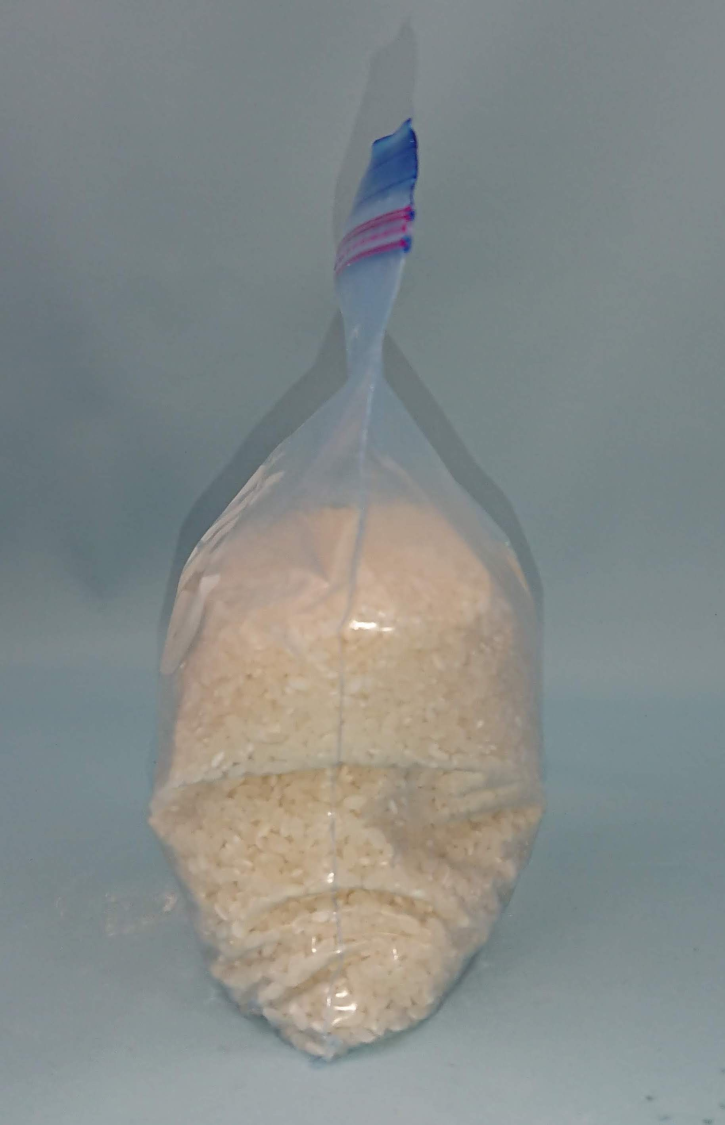
\includegraphics[width=0.26\linewidth]{images/rice_rightside.pdf}
 \label{fig:rice_rightside}} \\ 
\subfigure[Back view]{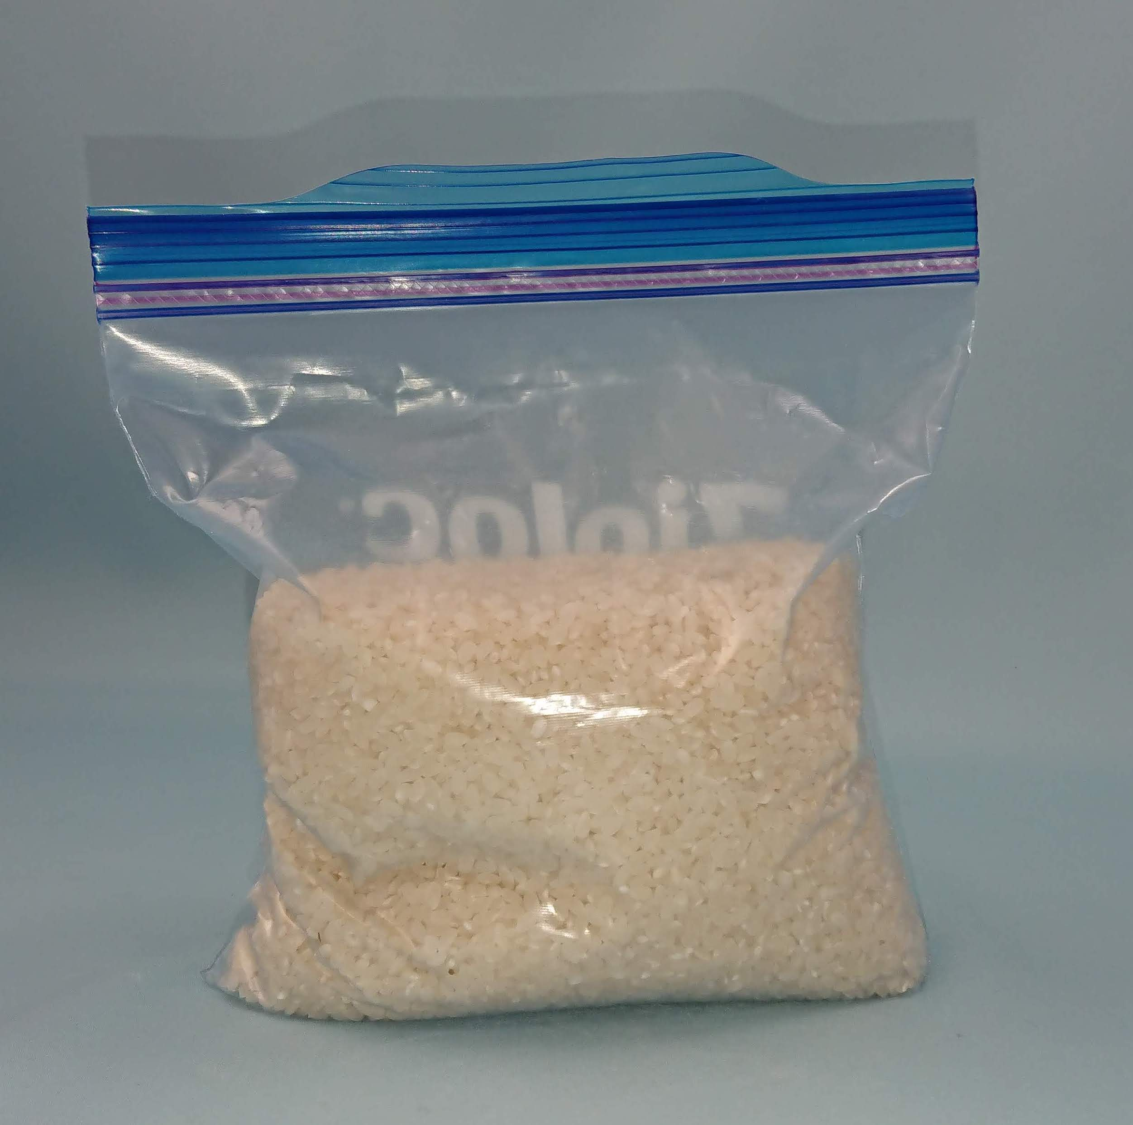
\includegraphics[width=0.46\linewidth]{images/rice_back.pdf}
 \label{fig:rice_back}} 
\subfigure[Top view]{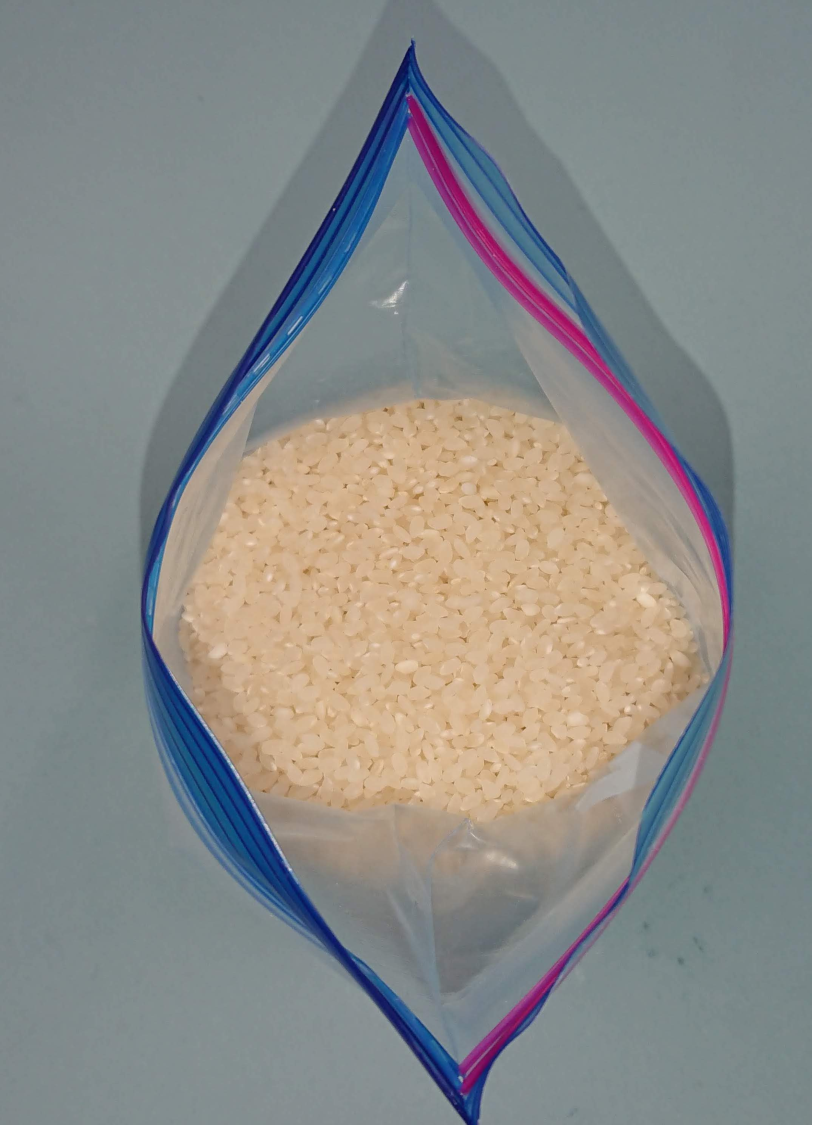
\includegraphics[width=0.35\linewidth]{images/rice_top.pdf}
 \label{fig:rice_top}}  
\caption{Appearance of rice}
\label{fig:rice}
\end{figure}

\newpage

